\documentclass[11pt]{article}
\setcounter{tocdepth}{3}
\setcounter{secnumdepth}{3}

\usepackage[english,italian]{babel}
\usepackage[a4paper, top=2cm, bottom=1.5cm, left=2cm, right=2cm]{geometry}
\usepackage{float}
\usepackage{ltablex}
\usepackage{titling}
\usepackage{blindtext}
\usepackage[utf8]{inputenc}
\usepackage[T1]{fontenc}
\usepackage{xcolor}

\usepackage{natbib}
\usepackage{graphicx}

\usepackage{geometry}
\usepackage[italian]{babel}
\usepackage{tabularx}
\usepackage{longtable}
\usepackage{hyperref}
\usepackage[bottom]{footmisc}
\usepackage{fancyhdr}
\usepackage{titlesec}
\usepackage{amsmath, amssymb}
\usepackage{array}
\usepackage{graphicx}
\usepackage{url}
\usepackage{comment}
\usepackage{eurosym}


\begin{document}

\thispagestyle{empty}
	\begin{titlepage}
		\begin{center}
			
\includegraphics[scale = 0.05]{Res/logo_unipd.png}\\
			\bigskip
			\large \textbf{Università degli Studi di Padova} \\
			\vfill
			
\includegraphics[scale = 0.7]{Res/BugPharma_Logo.png}\\
			\huge \textbf{Gruppo Bug Pharma} \\
			\vfill
			\large \texttt{bugpharma10@gmail.com}
			\vfill
			\Huge \textbf{Valutazione Capitolati 2021/2022}\\
			
			\vfill
			
			\large
			\begin{tabular}{r|l}
				\textbf{Approvazione} &  -\\
				\textbf{Redazione} &  \parbox[t]{3.5cm}{Lorenzo Piran \\ Michele Masetto \\ Sara Nanni \\ Andrea Salmaso}\\
				\textbf{Verifica} &  Nicholas Sertori\\
				\textbf{Stato} & Redatto \\
				\textbf{Uso} & Esterno
			\end{tabular}
			\vfill
			
		\end{center}
	\end{titlepage}

\tableofcontents

\newpage


\section{Valutazione del capitolato scelto}

\subsection{Capitolato C5 - Login Warrior}

    \subsubsection{Informazioni generali}
    \begin{itemize}
        \item \textbf{Nome}: Login Warrior;
        \item \textbf{Proponente}: Zucchetti S.p.A.;
        \item \textbf{Committente}: Prof. Tullio Vardanega e Prof. Riccardo Cardin.
    \end{itemize}
    
    \subsubsection{Descrizione}
    Il capitolato ha per oggetto l'affidamento della fornitura per la realizzazione di un'applicazione di visualizzazione di dati di
    login a supporto della fase esplorativa (\textit{EDA}) del riconoscimento e distinzione di attività lecite o illecite che possono
    essere svolte all'interno delle procedure cloud fornite dall'azienda ai propri clienti.
    
    Tale applicazione fornirà quindi ausilio ai data analyst, i quali, partendo da un insieme di dati contenuti in un file
    \texttt{CSV}, potranno risalire a grafici e dataset che forniranno un immediato riscontro visivo sulla presenza o meno di attività
    illecite, come riportato esemplificativamente in figura qui sotto:
    
    \bigskip
    
    \begin{figure}[h!]
        \centering
        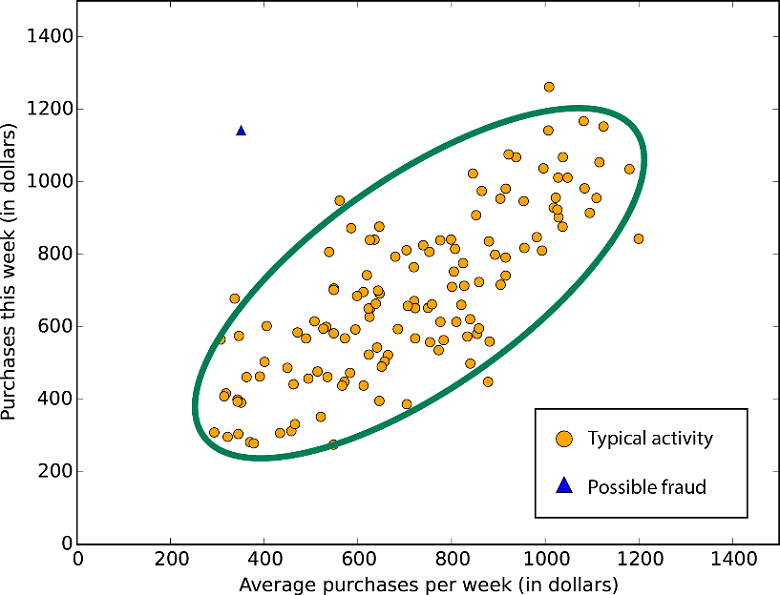
\includegraphics[scale=0.4]{Res/LoginWarrior.png}
        \caption{Esempio di un grafico raffigurante una possibile frode.}
        \label{zucchetti}
    \end{figure}
    
    \subsubsection{Dominio}
        \paragraph{Dominio applicativo}~\\
        
        \noindent
        Il capitolato si colloca nell'ambito della creazione di un applicativo web che permetta l'importazione di dataset presenti in
        file \texttt{CSV} e la visualizzazione di varie tipologie di grafico basate su di essi.
        Gli utenti finali sono quindi data analyst che analizzeranno gli accessi alle procedure cloud messe a disposizione dall'azienda.
        
        \paragraph{Dominio tecnologico}~\\
        
        \noindent
        Per lo svolgimento del capitolato e per la creazione dell'applicativo web vengono richieste conoscenze in ambito web, in
        particolare:
        \begin{itemize}
            \item \textit{HTML}: per la struttura ed il markup della pagina;
            \item \textit{CSS}: per la presentazione visiva dell'applicativo web;
            \item \textit{JavaScript}: per il comportamento e il trattamento dei dati;
            \item \textit{D3.js}: libreria \textit{JavaScript} per la manipolazione di documenti basati sui dati;
        \end{itemize}
    
    \subsubsection{Motivazione della scelta}
        \paragraph{Aspetti positivi}
        \begin{itemize}
            \item Le tecnologie e la libreria proposta da Zucchetti S.p.A sono strumenti molto diffusi e utilizzati nell'ambito della
            gestione e presentazione dei dati, con conseguente esaustività della documentazione;
            \item Consistente set di dati su cui effettuare test;
            \item Disponibilità mostrata dall'azienda all'aiuto e alla collaborazione con il gruppo, evidenziando quanto un eventuale
            risultato positivo possa essere effettivamente utilizzato in futuro;
            \item Possibilità di ottenere nuove conoscenze spendibili in futuro nel mondo lavorativo;
            \item Possibilità di applicare gli insegnamenti avuti dal corso parallelo di Tecnologie Web.
        \end{itemize}
        \paragraph{Fattori critici}
        \begin{itemize}
            \item La maggior parte degli elementi del gruppo ha poca o nulla familiarità con le tecnologie proposte;
        \end{itemize}
    
    \subsubsection{Conclusioni}
    Il buon esito degli incontri avuti con il referente di Zucchetti S.p.A., Gregorio Piccoli, e le accortezze prese dall'azienda,
    nonché la possibilità di utilizzare tecnologie interessanti e di affrontare un argomento molto stimolante per tutti gli elementi del
    gruppo, ha portato alla scelta del capitolato in oggetto.

\newpage


\section{Valutazioni sui capitolati rimanenti}

\subsection{Capitolato C1: Bot4Me}

    \subsubsection{Informazioni generali}
    \begin{itemize}
        \item \textbf{Nome}: Bot4Me;
        \item \textbf{Proponente}: Imola Informatica S.p.A.;
        \item \textbf{Committente}: Prof. Tullio Vardanega e Prof. Riccardo Cardin.
    \end{itemize}
    
    \subsubsection{Descrizione}
    Il capitolato si focalizza sulla realizzazione di un'applicazione chatbot in grado di interpretare un flusso testuale,
    con lo scopo di aiutare i dipendenti a familiarizzare con gli strumenti e con il contesto aziendale.
    
    \begin{figure}[h!]
        \centering
        
\includegraphics[scale=0.3]{Res/BotMe.png}
        \caption{Logo Bot4Me}
        \label{Bot4Me}
    \end{figure} 
    
    \subsubsection{Dominio}
        \paragraph{Dominio applicativo}~\\

		\noindent
        Il capitolato vuole soddisfare l'esigenza del poter consuntivare le attività giornaliere dei dipendenti aziendali in un
        periodo storico ove il Covid-19 ha costretto a mutare radicalmente modi di fare e abitudini delle persone.
        L'applicazione permetterebbe quindi di:
		\begin{itemize}
			\item Effettuare operazioni di check-in e check-out;
			\item Consuntivare l'attività giornaliera;
			\item Creare nuove riunioni;
			\item Aprire ticket di tracciamento di bug o progetti;
			\item Ricercare dei documenti sul repository aziendale;
			\item Aprire il cancello della sede aziendale.			
		\end{itemize}		        
		
        \paragraph{Dominio tecnologico}~\\
        
        \noindent
        Per lo svolgimento del capitolato e per la creazione dell'applicativo sono richieste la conoscenza e la padronanza
        delle seguenti tecnologie:
        \begin{itemize}
            \item \textit{API di EMT}: per la registrazione dell'ingresso e l'inserimento di attività;
            \item \textit{Protocollo MQTT}: per la gestione dell'apertura del cancello (requisito opzionale);
            \item \textit{API Redmine}: per effettuare le operazioni di inserimento di un nuovo ticket;
        \end{itemize}
    
    \subsubsection{Fattori critici}
    Qui di seguito i fattori critici sui quali si è soffermato il gruppo e che hanno fatto desistere dalla scelta del capitolato in
    oggetto:
    	\begin{itemize}
            \item Presenza di molti requisiti obbligatori, i quali richiedono una certa praticità con tecnologie differenti;
            \item Necessaria interpretazione del flusso vocale, oltre a quello testuale.
            \item Difficoltà nel garantire un alto livello di sicurezza senza poter richiedere l'autenticazione per lo strumento in uso;
        \end{itemize}
        
    \subsubsection{Conclusioni}
    Il dominio applicativo del capitolato appartiene ad un ambito che ha stimolato pochi membri del gruppo.
    Dopo un colloquio con l'azienda proponente, il gruppo ha rivalutato il proprio interesse per il capitolato in esame, riconoscendone il potenziale.
    Questo tuttavia non ha eliminato i dubbi già presenti per quanto riguarda la mole di lavoro richiesta e la scarsa conoscenza delle tecnologie coinvolte.
    
    \newpage


\subsection{Capitolato C2: BlockChange}

    \subsubsection{Informazioni generali}
    \begin{itemize}
        \item \textbf{Nome}: BlockChange - Exchange Platform on BlockChain;
        \item \textbf{Proponente}: Sync Lab S.r.l.;
        \item \textbf{Committente}: Prof. Tullio Vardanega e Prof. Riccardo Cardin.
    \end{itemize}
    
    \subsubsection{Descrizione}
	Il capitolato espone la richiesta di realizzazione di una piattaforma di pagamento digitale che utilizzi come metodo di pagamento
	un insieme di cripto valute. Lo scopo di tale servizio dovrebbe essere quello di garantire lo scambio di beni tra acquirente e
	fornitore in maniera sicura e affidabile, in modo tale che nessuna delle due parti sia lesa, sulla base dello schema riportato in
	figura qui sotto:
    
    \begin{figure}[h!]
        \centering
        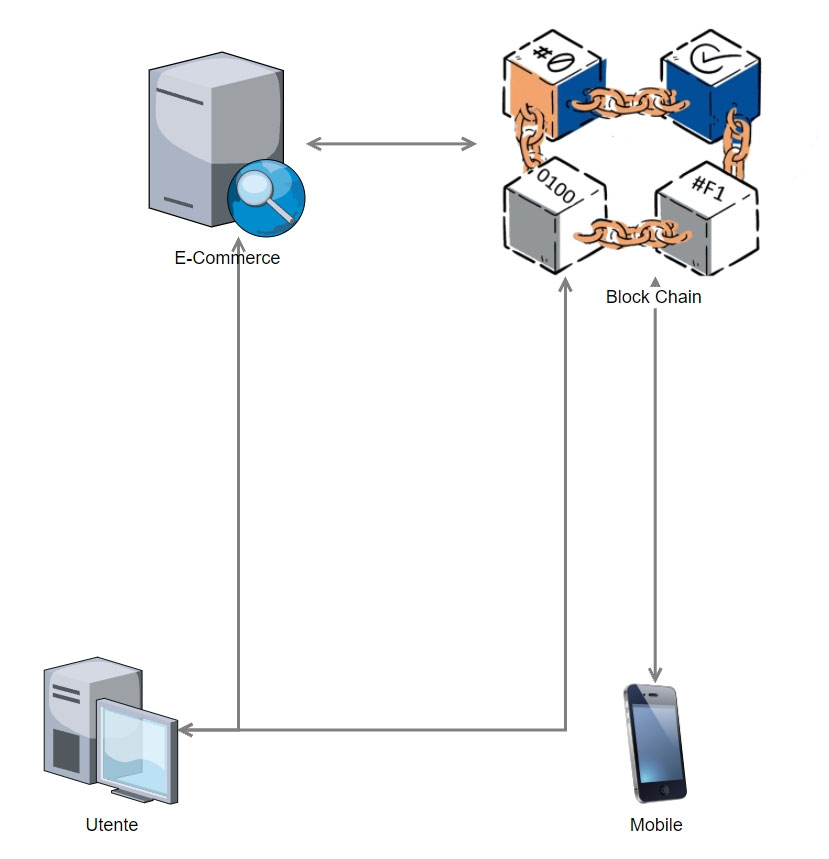
\includegraphics[scale=0.4]{Res/SyncLab.png}
        \caption{Schema della soluzione della piattaforma.}
        \label{SyncLab}
    \end{figure}
    
    \subsubsection{Dominio}
        \paragraph{Dominio applicativo}~\\
        
        \noindent
        Il capitolato si colloca nell'ambito degli acquisti online, ove da un lato è presente il compratore che desidera acquistare un
        bene mediante cripto valuta, mentre dall'altro il venditore che vende un prodotto.
        Il luogo in cui le due parti si incontrano è un e-commerce.
        
        \paragraph{Dominio tecnologico}~\\
        
        \noindent
        Il proponente preferisce non imporre tecnologie specifiche, ma resta aperto a nuove idee e proposte da parte dei fornitori.
        Tuttavia esprime alcune scelte preferenziali da considerare nello svolgimento del progetto:	
        \begin{itemize}
		    \item \textit{Ethereum}: come blockchain pubblica;
		    \item \textit{Solidity}: per la definizione degli smart contract;
			\item \textit{Java} e \textit{Angular}: per lo sviluppo delle parti di back-end e di front-end della componente
			web application del sistema;
			\item \textit{PostgreSQL}: per il database.
		\end{itemize}
    
    \subsubsection{Fattori critici}
    Qui di seguito i fattori critici sui quali si è soffermato il gruppo e che hanno fatto desistere dalla scelta del capitolato in
    oggetto:
   	\begin{itemize}
		\item Scarsa conoscenza da parte del gruppo in ambito blockchain così come della maggior parte delle tecnologie consigliate;
		\item Elevata quantità di casi d'uso di possibile difficile gestione.
	\end{itemize}
	
    \subsubsection{Conclusioni}
    La proposta in oggetto era stata inizialmente presa in considerazione dal gruppo. Tuttavia, durante gli incontri tenutisi tra i membri
    sono emerse perplessità riguardanti la sua effettiva fattibilità. Dato che l'incontro tenutosi con l'azienda ha risposto solo
    parzialmente ai dubbi, si è scelto di escludere questo capitolato. 
    
    \newpage


\subsection{Capitolato C3: CC4D}

    \subsubsection{Informazioni generali}
    \begin{itemize}
        \item \textbf{Nome}: CC4D;
        \item \textbf{Proponente}: SanMarco Informatica S.p.A.;
        \item \textbf{Committente}: Prof. Tullio Vardanega e Prof. Riccardo Cardin.
    \end{itemize}
    
    \subsubsection{Descrizione}
    Il capitolato ha per oggetto la creazione di: 
	\begin{itemize}
		\item Una web application che permetta all'utente (admin/configurator) di censire le macchine produttive e
		le relative caratteristiche da raccogliere e visualizzare;
		\item Una API (\textit{REST} o \textit{GraphQL}), per l'immissione della misurazione di una determinata
		caratteristica;
		\item Un motore di calcolo che, alla ricezione di una nuova misurazione (da relativa API), si occupi di metterla in
		relazione con le misurazioni precedenti al fine di calcolare se la serie di punti evidenza un processo "fuori controllo";
		\item Una web application che permetta di selezionare una o più delle caratteristiche censite, a parità di macchina,
		e visualizzi a rotazione la relativa carta di controllo.
	\end{itemize}	    

    \subsubsection{Dominio}
        \paragraph{Dominio applicativo}~\\
        
		\noindent
        Il capitolato verte sull'utilizzo di svariati strumenti e tecnologie per la creazione di un applicativo volto all'utilizzo
        in ambito industriale per la rilevazione di conformità, come illustrato nella descrizione del progetto.
        
        \paragraph{Dominio tecnologico}~\\

		\noindent
        Per lo svolgimento del capitolato e per la creazione dell'applicativo sono richieste la conoscenza e la padronanza delle
        seguenti tecnologie:
        \begin{itemize}
            \item \textit{Java} o \textit{NodeJS}: per la creazione della API e del motore di calcolo;
            \item \textit{React}, \textit{Angular} o \textit{VUE}: per la creazione della web application;
            \item \textit{Sql} o \textit{NoSql}: per il salvataggio delle configurazioni prodotte dalla web application;
            \item \textit{MongoDb} o \textit{MariaDb}: per il salvataggio delle informazioni prodotte dalla API;
            \item \textit{D3.js}: per la creazione dei grafici.
        \end{itemize}
    
    \subsubsection{Fattori critici}
    Qui di seguito i fattori critici sui quali si è soffermato il gruppo e che hanno fatto desistere dalla scelta del capitolato in
    oggetto:
    \begin{itemize}
    	\item Elevata quantità di temi in ambiti differenti che richiederebbero un buon approfondimento;
    	\item Elevata quantità di requisiti obbligatori;
    	\item Necessaria conoscenza di diverse tecnologie;
    \end{itemize}
    
    \subsubsection{Conclusioni}
    Il dominio applicativo del capitolato appartiene ad un ambito che ha stimolato pochi elementi del gruppo, non spingendolo
    verso la scelta del capitolato in esame, ritenuto comunque molto valido nella sua interezza.
    
\newpage


\subsection{Capitolato C4: Guida Michelin @ social}

    \subsubsection{Informazioni generali}
    \begin{itemize}
        \item \textbf{Nome}: Guida Michelin @ social;
        \item \textbf{Proponente}: ZERO12;
        \item \textbf{Committente}: Prof. Tullio Vardanega e Prof. Riccardo Cardin.
    \end{itemize}
    
    \subsubsection{Descrizione}
    Il capitolato espone la richiesta di realizzazione di una piattaforma simile ad una guida Michelin. Lo scopo principale è quello
    di creare una classifica dei luoghi di maggiore interesse analizzando vari contenuti prelevati dai social network \textit{Instagram}
    e \textit{TikTok} ed incrociando i risultati ottenuti con le recensioni online.
    
    A tale scopo, la piattaforma deve essere in grado di estrapolare dai social informazioni utili a determinare se un luogo è giudicato
    positivamente o negativamente, partendo da ciò che viene condiviso (come commenti testuali, messaggi vocali, immagini, ecc.).
    
    \subsubsection{Dominio}
        \paragraph{Dominio applicativo}~\\
        
        \noindent
        Il capitolato si colloca nell'ambito dei social network. Esso vuole offrire ai propri utenti una buona esperienza utilizzando
        l'enorme quantità di contenuti creati pubblicamente dagli utilizzatori dei suddetti social network.
        
        \paragraph{Dominio tecnologico}~\\
        
        \noindent
        Il committente raccomanda di utilizzare la tecnologia \textit{Amazon Web Services}, in particolare:
		\begin{itemize}
			\item \textit{AWS Fargate}: servizio serverless per la gestione a container;
			\item \textit{AWS AppSync}: servizio gestito per lo sviluppo rapido di API \textit{GraphQL};
			\item \textit{Neptune}: database a grafo ideale per tracciare efficientemente le relazioni tra i dati.
		\end{itemize}
		Sono inoltre richieste la conoscenza e la padronanza delle seguenti tecnologie:
		\begin{itemize}
			\item \textit{NodeJS}: per lo sviluppo di API Restful \textit{JSON} a supporto dell'applicativo;
			\item \textit{Swift}: per lo sviluppo di app in ambito \textit{iOS}/\textit{MacOS};
			\item \textit{Kotlin}: per lo sviluppo di app in ambito\textit{Android};
			\item \textit{Architettura a micro-servizi}.
		\end{itemize}
    
    \subsubsection{Fattori critici}
    Qui di seguito i fattori critici sui quali si è soffermato il gruppo e che hanno fatto desistere dalla scelta del capitolato in
    oggetto:
    \begin{itemize}
    	\item Iniziale scetticismo da parte del gruppo sulla possibilità di raccolta dei dati degli utenti, sulla base
    	delle normative sui dati vigenti di \textit{Instagram} e \textit{TikTok};
		\item Elevata complessità che potrebbe portare ad un progetto particolarmente dispendioso in termini di tempo;
		\item Poca familiarità con \textit{AWS}.
    \end{itemize}
        
    \subsubsection{Conclusioni}
    Il capitolato in oggetto non è stato considerato nelle scelte iniziali e finali del gruppo a causa dell'idea di fondo, considerata
    ancora troppo abbozzata, seppur molto interessante. Sono emersi inoltre dubbi sull'effettiva utilità dell'applicazione.

\newpage




\subsection{Capitolato C6: Smart4Energy}

    \subsubsection{Informazioni generali}
    \begin{itemize}
        \item \textbf{Nome}: Smart4Energy - A new way in energy monitoring and control;
        \item \textbf{Proponente}: Socomec Innovative Power Solutions;
        \item \textbf{Committente}: Prof. Tullio Vardanega e Prof. Riccardo Cardin.
    \end{itemize}
    
    \subsubsection{Descrizione}
    Il capitolato si focalizza sulla realizzazione di un ausilio ad un avanzamento tecnologico dei gruppi di continuità (UPS), per far si
    che possano essere fruiti ed utilizzati, tramite diverse tecnologie, da differenti device. Lo scopo, attraverso esso, è quindi quello
    di cambiare il modo in cui le persone si interfacciano ai dispositivi proprietari Socomec e il modo in cui ne verrebbe erogato il
    servizio di assistenza.
    
    \subsubsection{Dominio}
        \paragraph{Dominio applicativo}~\\
        
        \noindent
        Il capitolato vuole soddisfare una nuova esigenza nell'ambito della gestione degli UPS, derivata dai consumatori, proponendo
        all'utente una nuova esperienza d'uso tramite il proprio dispositivo personale (smartphone o tablet), così da metterlo naturalmente
        a suo agio.
        
        \paragraph{Dominio tecnologico}~\\
        
        \noindent
        Per lo svolgimento del capitolato e per la creazione dell'applicativo che si interfaccerebbe con l'unità di UPS, il proponente
        preferisce non imporre vincoli, pur consigliando la scelta di una tecnologia/architettura che possa coprire il più possibile i
        requisiti richiesti e opzionali.
        
        Essendo i devices odierni quasi totalmente dotati di sistema operativo \textit{Android} e \textit{iOS}, le tecnologie di sviluppo
        potrebbero corrispondere a:
        \begin{itemize}
            \item \textit{Kotlin}: per la parte di programmazione relativa ad \textit{Android};
            \item \textit{Swift}: per la parte di programmazione relativa ad \textit{iOS};
        \end{itemize}
        
        Il proponente richiede almeno:
        \begin{itemize}
        	\item \textit{GitLab}: per l'apertura di un progetto privato di cui verranno fornite le credenziali;
        \end{itemize}
    
    \subsubsection{Fattori critici}
    Qui di seguito i fattori critici sui quali si è soffermato il gruppo e che hanno fatto desistere dalla scelta del capitolato in
    oggetto:
    \begin{itemize}
            \item Poca familiarità con con le tecnologie proposte;
            \item Capitolato potenzialmente troppo lungo e dispersivo.
        \end{itemize}

    \subsubsection{Conclusioni}
    Il dominio applicativo del capitolato appartiene ad un ambito che ha stimolato pochi elementi del gruppo, non spingendolo
    verso la scelta del capitolato in esame, ritenuto comunque molto valido nella sua interezza.

\end{document}
